\section{Business Analytics} 

\vspace{16mm} %5mm vertical space
\begin{center}
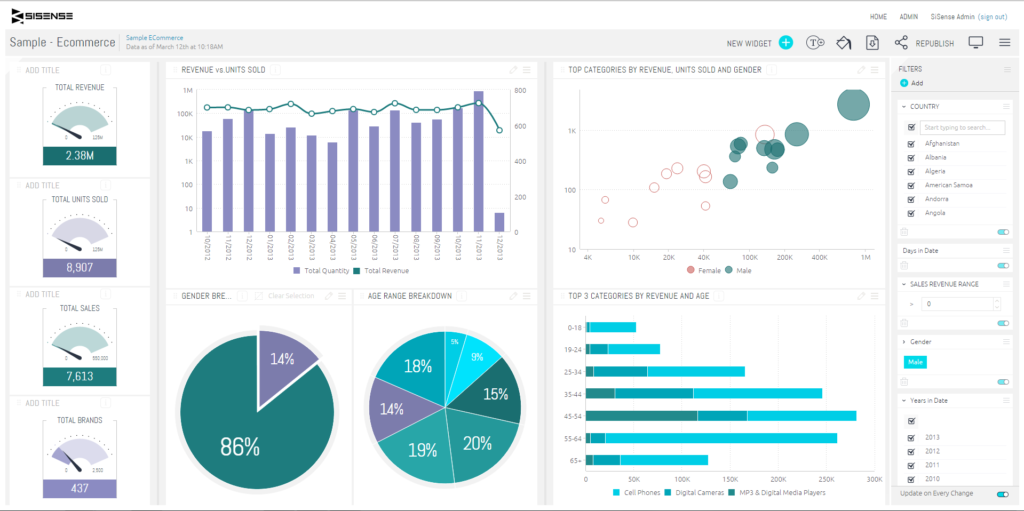
\includegraphics[width=17cm]{./Imagenes/002}
\end{center}	
\vspace{12mm} %5mm vertical space

Al igual que la inteligencia empresarial, BA recopila y analiza datos, emplea el análisis predictivo y genera informes ampliamente visualizados en tableros personalizados. El objetivo de estas características es ayudar a identificar y abordar los puntos débiles de una organización. Aquí es donde terminan las similitudes. El software de análisis empresarial se utiliza para explorar y analizar datos históricos y actuales. Utiliza el análisis estadístico, la minería de datos y el análisis cuantitativo para identificar las tendencias comerciales pasadas.\\
Una vez que se han recopilado y analizado los datos, los sistemas de análisis de inteligencia empresarial luego usan esa información para el modelado predictivo. Esto puede predecir y, en la mayoría de los casos, prepararse para los climas comerciales futuros. Uno de los aspectos más potentes de BA es la generación de informes ad hoc, que permite a las empresas realizar análisis de datos específicos en tiempo real para responder preguntas específicas y tomar decisiones comerciales más rápidas. En efecto, el análisis empresarial usa el análisis predictivo para resolver problemas antes de que ocurran.\\
BA es una expresión general para los enfoques y las tecnologías que puede utilizar para acceder y explorar los datos de su empresa, con el fin de extraer nuevos conocimientos útiles para mejorar la planificación empresarial y aumentar el rendimiento futuro.

